
\chapter{语言模型实验结果与分析}
在前面两章中,我们分别介绍了树状分层概率计算模型和类别层次概率计算模型的具体建模过程。在本章中,为了比较所提出的分层并行概率计算模型与已有的计算模型方法(Baselines)的效率和准确性,我们将在三个标准文本数据集:Wikitext-2,Wikitext-103 和 One Billion Word数据集上,进行了循环语言建模任务的实验研究和实验结果分析。本文将会展示并行层次概率计算算法的实验结果,我们还会与其他大词表问题的优化加速算法相互对比。 此外,我们还将从效率分析、可扩展性、参数大小和性能等四个方面,对这些已有的方法进行实验研究并作讨论分析。

\section{实验设置}
在这一小节,我们将介绍实验所需要用到的文本数据集,语言模型实验的两种主要的评测指标和实验模型的实际训练参数配置和训练过程。
\subsection{实验数据集}
本次实验所采用的数据集主要是依照两个目的选取的:我们需要在小数据集能反映参数变化对模型的最后的效果产生的影响,同时我们还需要大数据集展示模型参数在最佳配置下模型的最优结果比较情况。所以在本次实验中,我们选取了三个标准文本数据集:Wikitext-2,Wikitext-103 和 One Billion Word数据集。
如表~\ref{tab:dataset}~所示,表中列举了这三个数据集全部统计指标:单词数量、句子数量、词表大小和词表外单词的比例(Out-of-Vocabulary)。这里我们需要注意的是,我们不能改变词表大小,而且不同词表大小的模型之前理论上是没有互相比较的意义的。
因为我们接下来要计算的一个重要的评测指标就是和词表大小成负相关关系的。
所以表~\ref{tab:dataset}~中展示的数据已经预先固定了,不会再做任何的修改,例如:单词大小写变化,数词转换操作或者分词操作。
\begin{table}
  \centering
  \caption{WikiText-2, WikiText-103 和 One Billion Words 数据集统计指标 \label{tab:dataset}}
\begin{tabular}{llrrrrr}
\toprule
数据集& 类型& 文章数 & 句子数量 &  单词数量 &词表大小 & OOV (\%) \\ \midrule
\multirow{3}{*}{Wikitext-2} &训练集& 600 & 36,718 & 2,088,628 & \multirow{3}{*}{33,278} & \multirow{3}{*}{2.6\%} \\
&验证集& 60 &3,760 & 217,646  & &\\
&测试集& 60 & 4,358 & 245,569 & &\\
\midrule
\multirow{3}{*}{Wikitext-103} &训练集& 28,475 &  1,801,350 &  103,227,021 & \multirow{3}{*}{267,735} & \multirow{3}{*}{0.4\%} \\
&验证集& 60 &3,760 & 217,646  & &\\
&测试集& 60 & 4,358 & 245,569 & &\\
\midrule
\multirow{3}{*}{One Billion Word} &训练集& --- &30,301,028&768,646,526&   \multirow{3}{*}{793,471} &   \multirow{3}{*}{0.28\%} \\
 &验证集& --- &  6,075 &   153,583 &&\\
 &测试集 & --- &  6,206 &   159,354 &&\\
\bottomrule
\end{tabular}
\end{table}

其中,对于~Wikitext-2和Wikitext-103~数据集,训练、验证和测试集都是预先划分固定的,并且其词汇表大小也已经被定义\footnote{https://metamind.io/research/the-wikitext-long-term-dependency-language-modeling-dataset/}。
这两个数据集拥有相同的验证和测试集,而Wikitext-103的训练集则比Wikitext-2的训练集大得多。所以我们还可以间接测算出增大训练集对测试集上的提升效果表现。对于第三个``One Billion Word''数据集\footnote{http://www.statmt.org/lm-benchmark/},它是由之前机器翻译数据集里面的的文本融合而成,文本数据也取自维基百科(Wikipedia)\footnote{英文维基百科主页:https://en.wikipedia.org/wiki/Main\_Page/}。
为了评价的标准性和实验的可互相比较性,官方还提供了一套数据预处理脚本,同时指定了该脚本所需要的~Perl~语言版本,可见要求极为严苛。因为对于语言模型来说,Perl~内置函数处理出来的文本也略有不同,语言模型之间的结果相互比较就会变得没有意义的。通常来说,词表小的模型更占优势。当我们用官方提供的脚本处理完数据后,我们将``./train/''目录中的所有数据视为训练集,选择``./holdout/''目录下面的第一和第二个数据集作为相应的验证和测试集。这些数据集的详细统计指标在表~\ref{tab:dataset}~中进行了详细说明。

\subsection{实验评价指标}
在本次实验研究中,当我们将各种实验模型在训练数据集上训练到收敛之后,我们就需要评价不同模型的性能差异,针对语言模型的两个标准评估度量标准来揭示针对不同的优化方法的优劣:困惑度(Perplexity,$ \mathrm{PPL} $)和单词误差率(Word Error Rate,$\mathrm{WER} $)。
其中,$ \mathrm{PPL} $是一个内在度量指标(Intrinsic Metric),代表了在候选人中选择下一个话语时的混乱程度。语言模型较低的困惑意味着在相同词表下拥有更好的可预测性。此外,在整个测试集上,$\mathrm{PPL}$ 数值是与平均负对数似然值(NLL)呈指数相关关系,表示我们训练过程中我们直接优化了我们的评测指标,即困惑度量。
\begin{equation}\label{equ:ppl}
   \mathrm{PPL}(w_1,\cdots,w_T)=\sqrt[T]{\frac{1}{\prod_{t=1}^T p(w_t|w_{1:t-1})}}
\end{equation}

此外,$\mathrm{WER}$指代的是单词的萊文斯坦距离(Levenshtein Distance),于衡量两个字符串参考句子(reference,记作r)和预测句子(hypothesis,记作h)之间的相似度。他是编辑距离的一种衍生出来的类型,它被定义为错误识别的单词(删除,插入,替换)占单词总数的百分比\footnote{https://martin-thoma.com/word-error-rate-calculation}:
\begin{equation}\label{equ:wer}
  \mathrm{WER} = \frac{\text{插入的单词数 + 删除的单词数 + 替换的单词数}}{\text{全部单词数量}}
\end{equation}
其数学形式的定义公式为:
\begin{equation}\label{equ:distance}
d_{r,h}(i,j) =  \begin{cases}
\max (i,j)& \text{如果}\min(i,j)=0\\
\min  \begin{cases}
d_{r,h}(i - 1,j) + 1,\text{//插入的单词}\\
d_{r,h}(i,j - 1) + 1,\text{//删除的单词}\\
d_{r,h}(i - 1,j - 1) + I{(r_i\neq h_j)},\text{//替换的单词}
\end{cases} &\text{否则}
\end{cases}
\end{equation}
其中$I{(r_i\neq h_j)}$ 指代的是示性函数, 当且仅当$r_i= h_j$的时候取值为$0$,否则该函数取值为$1$。 $d_{r,h}(i,j)$ 表示的是参考句子 $r$的第一个$i$个字符与预测句子 $r$的第一个$j$个字符之间的距离。

我们在本实验中采用萊文斯坦距离作为我们的一个度量指标,主要是考虑到该距离度量的延展性(三角不等式)。 两个字符串的距离不大于分别与第三个字符串的距离之和:
\begin{equation}
d_{r,h}+d_{r,s}\ge d_{r,s}
\end{equation}
其中 $s$ 代表另外一个生成的句子,$d_{r,h}$表示的是句子~r~和句子~h~之间的编辑距离。

除了以上的定量的度量指标,\textit{训练时间效率,词汇可伸缩性}和\textit{运行时内存消耗}等定性度量指标也应该被视为衡量不同模型的重要衡量维度。因此,我们在实验中分别从GPU和CPU的理论和经验角度分析了不同优化算法在不同评估指标上的具体数值结果。最后,统计实验数值并分析在三个标准文本数据集上的最终结果。

\subsection{模型训练和参数配置}
接下来我们来介绍实验模型的参数设置和训练方法。在我们的实验研究中,每个模型都是使用Theano框架实现的而且都运行在一个独立的GPU设备上,它具有12GB的显存(即Nvidia K40m),使得大矩阵乘法的运算成为可能,也就是说我们能测试大词表的计算代价。然而,我们在实际试验中发现随着参数维数的增加,一个GPU显存资源被快速利用殆尽。

然后,对于wikitext-2数据集来说,我们固定最大句子长度为256;对于wikitext-103数据集来说,我们固定最大句子长度为100;对于OBW数据集来说,我们固定最大句子长度为50,因为它词表最大,需要占用更多的显存消耗。对于长度超过长度阈值的那部分字符串,超出部分全部删除。由于我们测量的是语言模型的单词级损失(Word-Level Loss)而不是句子级的分数(Sentence-Level Loss),因此删除部分的那句子对模型训练的影响是很小的。
\begin{figure}[!t]
  \centering
  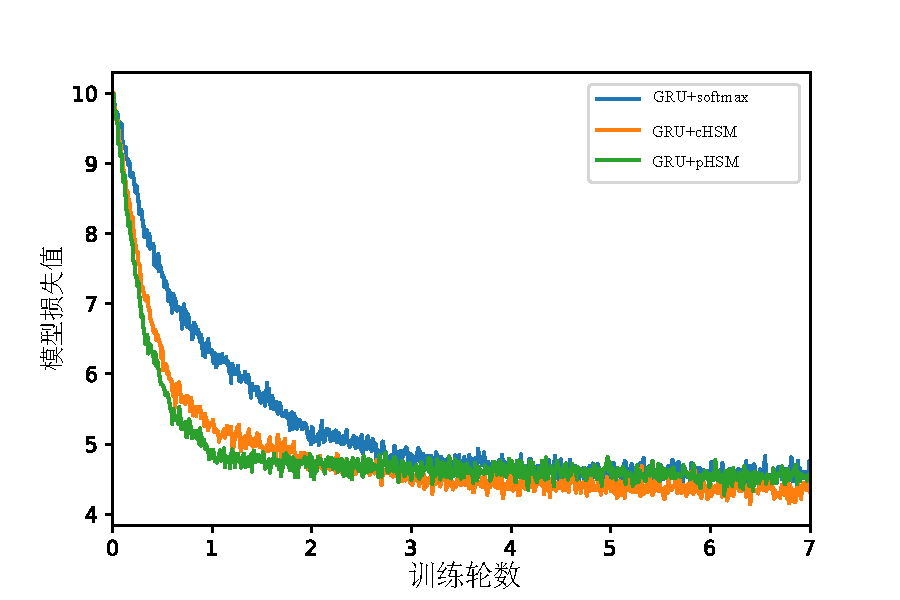
\includegraphics[width=0.6\columnwidth]{./figures/learn2.pdf}
  \caption{模型训练曲线图}
\end{figure}

另外,我们实验中采用Adam优化器(Optimizer)配合两种不同的学习率(Learning Rate),即设置$ lr = 0.06$ 和 $0.001 $。对于两种词表层级分解方法,我们将应用较大的学习率;而对于传统的softmax和采样近似方法,我们应用较小的学习率。因为我们实验中发现,词表层级分解算法收敛地很慢,需要配合更大的学习率。除此以外,每隔一定步数,我们还需要衰减学习率的大小:$lr \leftarrow lr *0.9$。

对于在WikiText-2数据集上运行的实验,我们在批处理大小(batch size)为20的20个时期内运行,直到我们观察到验证集上的最小$ \mathrm{PPL} $。验证集上的损失数值约4.8,这是最好的验证上的损失值。而对于Wikitext-103数据集,在训练集上优化参数需要大约3-4个轮数(Epochs),因为训练集大约比较小的一个大50倍。此外,训练集损失数值大约在5.1左右,因为在 wikitext-2 数据集上更高的原因是我们预测的词汇量要大得多,所以混淆程度(即训练损失)应该更高。虽然我们发现模型可以很容易地收敛到局部最小点,验证误差在这个局部最小值的范围内振荡,但是Wikitext-2和Wikitext-103的唯一区别是训练数据的大小,表示收集很多训练数据不一定能保证模型在相同的验证和测试集上学得更好,而不是更普遍的结果。

此外,我们在实验中发现在 OBW 数据集上运行实验相当具有挑战性,因为它需要更大的参数来拟合。所以我们应用优化的CUDA实现的RNN模型~\upcite{DBLP:journals/corr/AppleyardKB16},将RNN模块所需要的计算时间降到最低。然而,等待模型收敛到训练集上需要480小时,因此我们可以在验证集上得到可能的结果。

\section{影响因素比较}
我们在这部分将讨论语言模型的大词表问题的具体实验计算瓶颈和各种不同计算策略对实验计算效率和性能的影响。
\subsection{词表层次化比较}
我们首先使用wiki103数据集,统计了语言模型中每个模块的计算时间消耗,如图~\ref{fig:rnn_timing}~所示。 我们计算运行不同的RNN模型(即LSTM模型和GRU模型)及其梯度(即,RNN Grad)所需的时间,以及Wikitext-103数据集的大词汇表上的常规softmax,这词汇表大小与我们平时所采用的数据集的词表相当。 我们分别用Theano框架和CUDA实现了RNN单元,一个采用python语言实现,第二个使用并行C++语言实现。目前基于CuDNN实现的RNN模型计算时间最快,它里面的RNN的运行时间可以缩短到最短。 我们将代码重复了100遍,统计了每个模块的总时间占用,然后分别计算其平均时间占用。这样做的目的是通过多次实验来保证实验数据准确性。

从图中可以看出,使用优化的CUDA,softmax模块的影响比RNN单元及其梯度更重要。Softmax计算时间占用总计算时间随着词表的增大占比越来越大,并且已经超过了$50\%$的计算时间,这就需要我们详细讨论softmax优化。


\begin{figure}[!t]
  \centering
  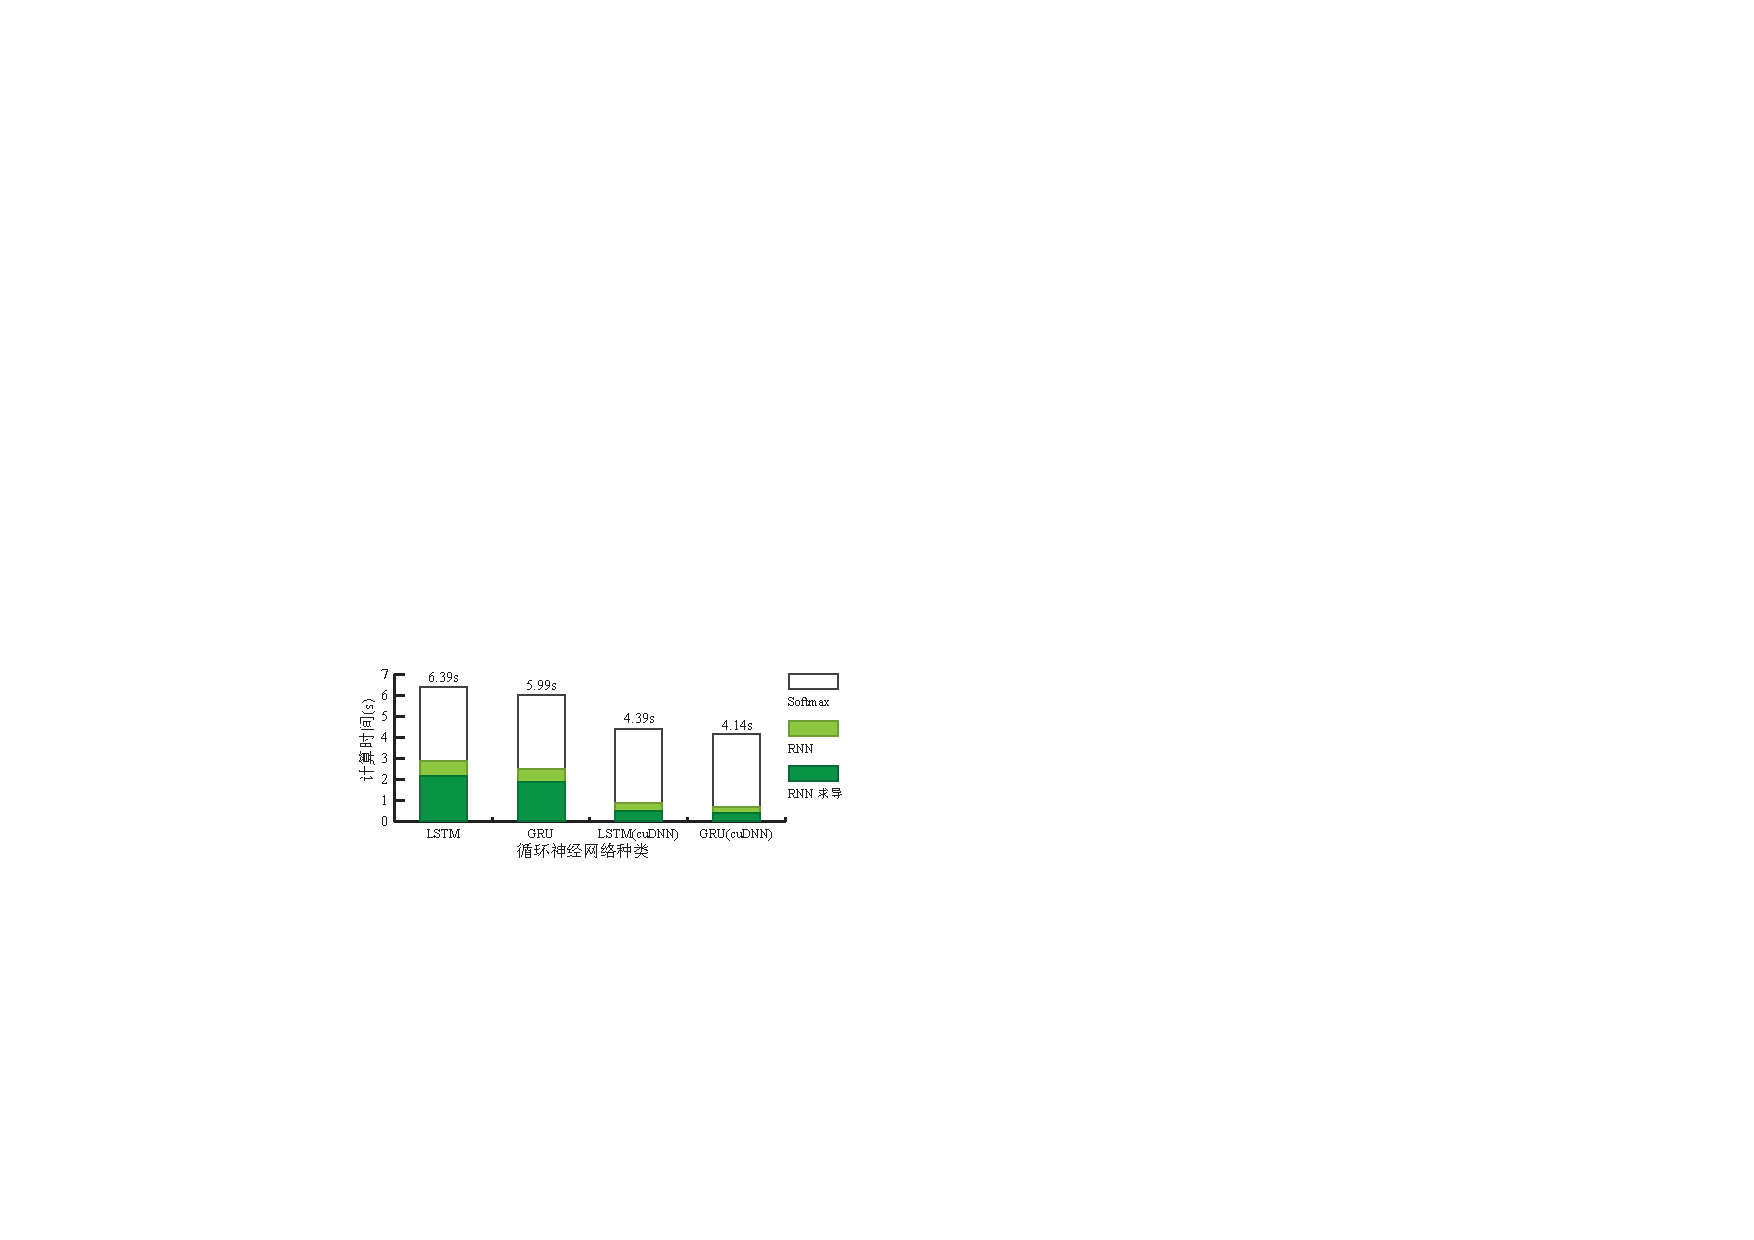
\includegraphics[width=.9\columnwidth]{./figures/rnn_timing.pdf}
  \caption{wikitext-103数据集上测量语言模型三个部分的计算时间比较}\label{fig:rnn_timing}
\end{figure}
\begin{figure}[!t]
  \centering
  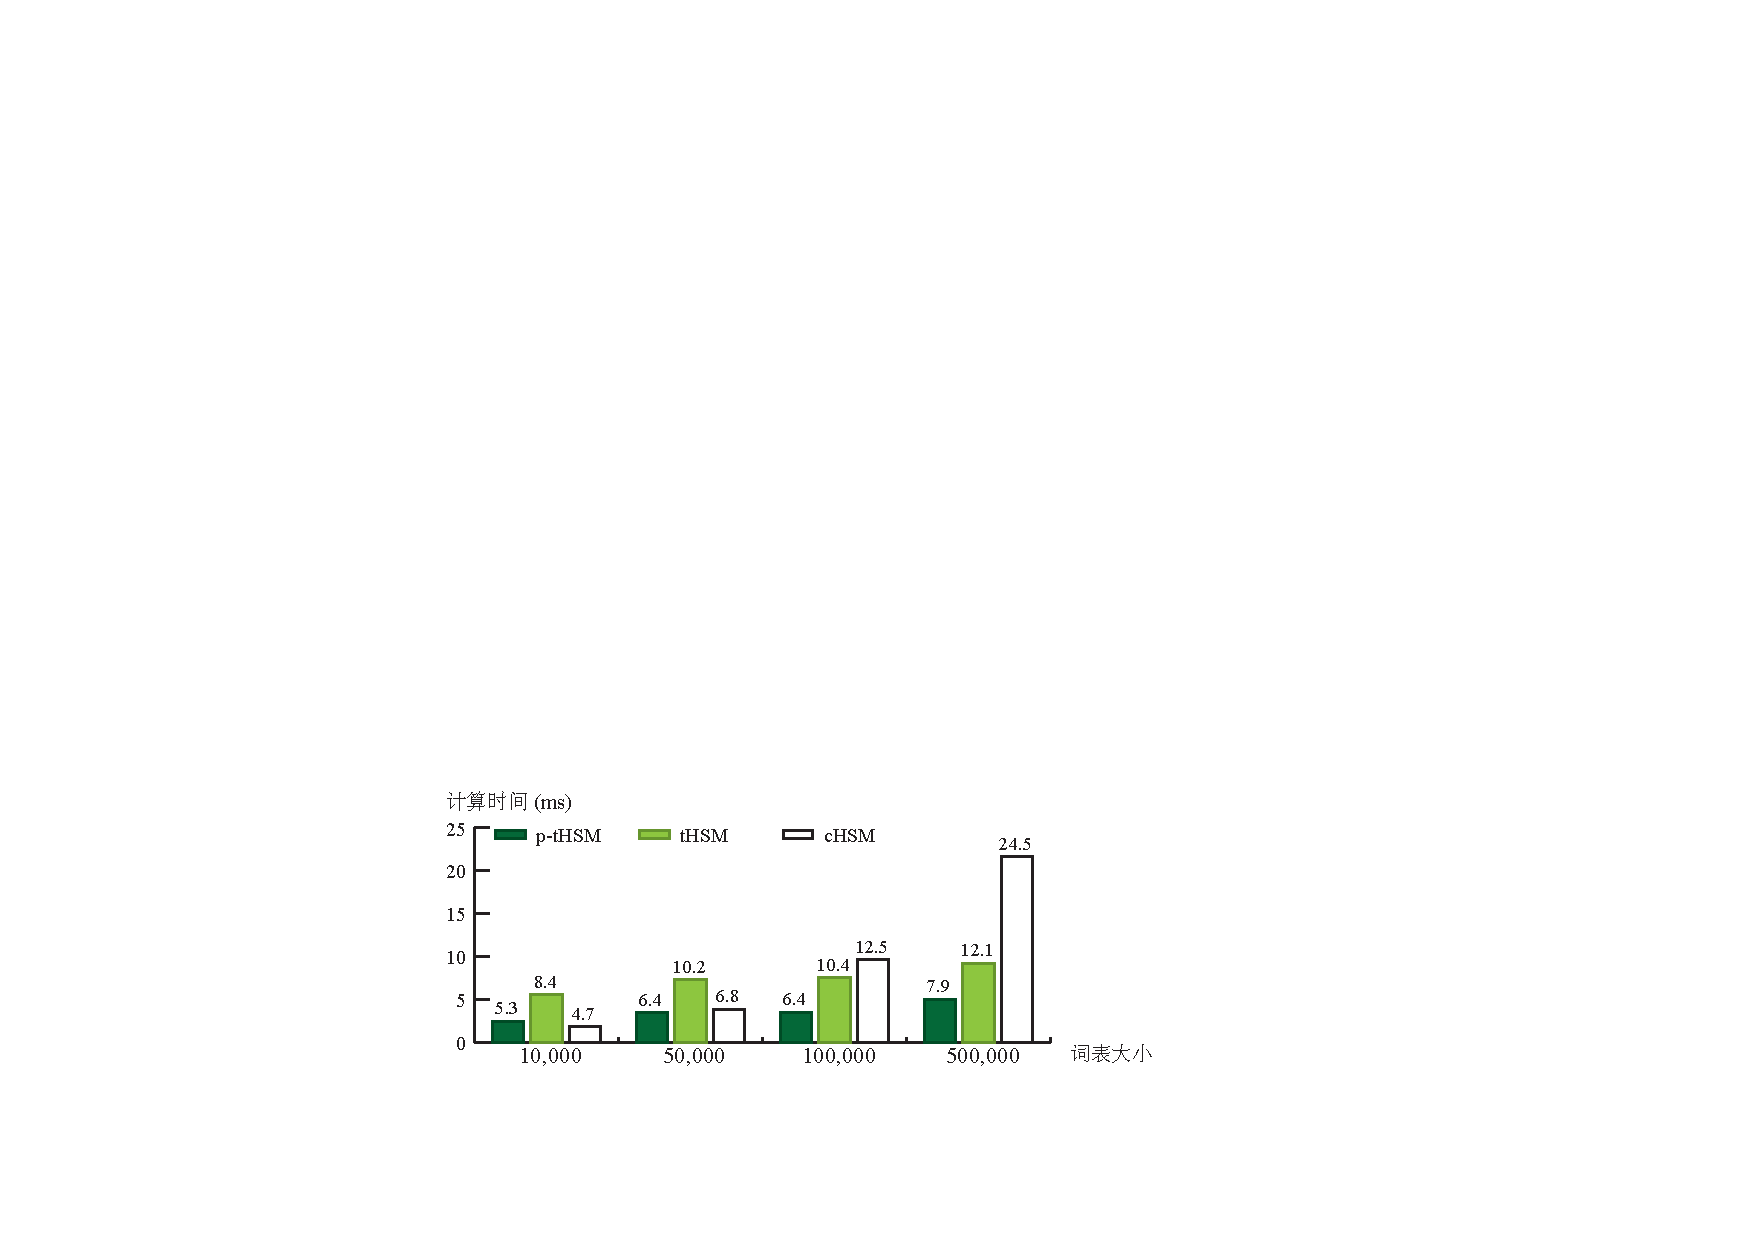
\includegraphics[width=.87\columnwidth]{./figures/all_time.pdf}
  \caption{cHSM, tHSM 和 p-tHSM 算法随着词表大小的计算时间影响}\label{fig:hsm_benchmark}
\end{figure}

为了对用于训练相同批处理数据的经验时间复杂性和内存消耗进行基准测试,我们使用这些算法在表~\ref{tab:time}~中收集了GPU和CPU上的详细结果。我们尝试使用这些算法处理WikiText-103数据集,并计算处理一个批处理数据所需的平均时间。另外,输入句子的最大长度,隐藏层,输出词汇和批量大小分别设置为$\{50, 256, 267735, 20\}$。此外,“总时间”过程表示前向传播和后向梯度优化的过程,“前进时间”过程表示从输入数据到计算模型成本所需的时间消耗。此外,我们计算了上述算法训练期间加载所需的内存。 $ \mathcal{| V |} $表示词汇大小,$ \mathcal{| H |} $是目标嵌入维度。在训练期间,tHSM只消耗最小的存储器资源,而p-tHSM覆盖了更大的存储器集合,并且p-tHSM在考虑存储器消耗和速度时采用更大的存储器并且获得了更好的加速比。

\begin{table}[!ht]
  \centering
  \caption{wikitext-103数据集上面GPU和CPU的运行时内存和计算时间比较\label{tab:time}}
\begin{tabular}{lccccc}
  \toprule
 \multirow{2}{*}{算法}  &\multirow{2}{*}{运行时内存占用} &\multicolumn{2}{c}{总计算时间 (ms)} & \multicolumn{2}{c}{前向计算时间 (ms)}   \\
   \cmidrule(lr){3-4}  \cmidrule(lr){5-6}
	& & CPU&GPU & CPU& GPU \\ \midrule
Softmax & $\mathcal{|HV|}$ &510.4  &262.1&352.2& 62.9 \\
cHSM    & $2\mathcal{|H|\sqrt{|V|}}$&506.5  &\textbf{40.6}&28.7&14.6 \\
tHSM    &$\mathcal{|H|}$&1,004.0 &444.4 & 8.1&  5.6   \\
p-tHSM  &$\mathcal{|H|\log{|V|}}$ &\textbf{383.5}&	86.4 &\textbf{7.0}&	\textbf{1.4} \\
  \bottomrule
\end{tabular}
\end{table}



为了验证与词汇大小相关的cHSM,tHSM和p-tHSM算法的可扩展性,结果展示在图~\ref{fig:hsm_benchmark}~中。 为了显示p-tHSM算法的影响,我们在这里不包含“Softmax”方法,因为与其他算法相比,它消耗了更多的计算时间,无法被放在这个图里面。 很显然,cHSM随着词汇大小的平方根(即,$ \mathcal{O(| H | \sqrt{| V |})} $)进行缩放,而p-tHSM随着词汇大小的增加呈现出稳定的表现。tHSM算法随着此表大小的对数进行变化 (即,$ \mathcal{O(| H | \log{| V |})} $),我们的p-tHSM算法所需要的计算时间词表变大,与tHSM算法的差异越来越大。这一结果证明我们提出的计算模型更加优越。


在这些实验的基础上,我们可以得出结论:所提出的p-tHSM方法胜过历史记录$ \mathcal{O(| H | \log| V |)})$,并且取得了令人满意的分层softmax方法的加速比。 这种性能归因于基于GPU并行性的加速,也是由于p-tHSM 方法的基本结构,能够将目标字树进行并行地计算。


\subsection{搜索策略的影响}
由于我们提出了三个关于推理阶段搜索策略的算法,其影响可以通过WER度量来观察。在这个结构化预测过程中,一个合适的搜索规则将帮助模型获得最小风险的最佳候选人,如表~\ref{tab:search}~所示。 “Global”方法表示我们计算所有单词的得分,单词的概率用整个词汇全局归一化。值得注意的是,对于cHSM方法算法~\ref{alog:greed_argmax}~比算法~\ref{alog:exact}~得到更好的WER,尽管后一种方法获得了词汇表上的确切顶级候选。由于类结构中存在标签偏差问题,排名最高的词容易出现算法模型无法建模的小组。最后但并非最不重要的是,算法~\ref{alog:exact}~和``global''获得相同的单词排序,唯一的区别是算法~\ref{alog:exact}~避免了冗余计算。所以他们达到了可比的WER得分,但算法~\ref{alog:exact}~需要更少的时间。
\begin{table}[!t]
  \centering
  \caption{wikitext-2数据集上ctHSM算法针对不同搜索算法的WER评测结果\label{tab:search}}
\begin{tabular}{llccc}
  \toprule
   & 算法&计算时间 (ms)&验证集 (WER)& 测试集(WER)\\ \midrule
  \multirow{3}{*}{cHSM} &global&102& 80.00\%& 80.02\%\\
        &算法~\ref{alog:exact}&63& 80.00\%& 80.02\%\\
        &算法~\ref{alog:greed_argmax}&\textbf{44}&\textbf{ 77.09\%}&\textbf{ 77.07\%}\\
  \bottomrule
\end{tabular}
\end{table}

\begin{table}[!t]
  \centering
  \caption{wikitext-2数据集上p-tHSM算法针对不同搜索算法的WER评测结果\label{tab:psearch2}}
\begin{tabular}{llccc}
  \toprule
        & 算法&计算时间 (ms)&验证集 (WER)& 测试集(WER)\\ \midrule
  \multirow{2}{*}{p-tHSM}  &global&161& \textbf{76.67\%}&\textbf{75.35\%}\\
        &算法~\ref{alog:greed_argmax}&\textbf{30} & 79.61\%&79.32\%\\
  \bottomrule
\end{tabular}
\end{table}

对于p-tHSM系列算法,我们比较了所提出的算法~\ref{alog:greed_argmax}和传统的“全局”算法。算法~\ref{alog:greed_argmax}比“global”方法获得本地最佳结果花费的时间更少。由于基于树的模型在以前的决策中更容易失败,所以“全局”方法的MER分数要比算法~\ref{alog:greed_argmax}要好。

\subsection{循环网络模型的影响}

从表~\ref{tab:rnn}~中可以看出,门控单元(即LSTM和GRU单元)的RNN模型在复杂度和字误码率方面比传统的RNN Relu和RNN Tanh模型表现得更好。因为门控功能可以避免梯度消失的问题。虽然它需要稍微多一些的时间进行计算。此外,LSTM的计算公式在GPU上比GRU单元更容易并行运行,因此LSTM比GRU模型需要更少的推理时间。
\begin{table}[!t]
  \centering
  \caption{wikitext-2数据集上不同循环网络针对 PPL、 WER和计算时间的影响\label{tab:rnn}}
\begin{tabular}{lccc}
  \toprule
  循环神经网络 & 计算时间 (ms)&验证集(PPL / WER) & 测试集(PPL / WER)\\ \midrule
  1$\times$RNN Relu~\upcite{DBLP:journals/jmlr/GutmannH10} &176.4&260.52 / 80.00\%&238.75 / 80.02\%\\
  1$\times$RNN Tanh~\upcite{DBLP:journals/iclr/JiVSAD15}   &176.2&250.57 / 79.61\%&230.98 / 79.32\%\\
  1$\times$LSTM~\upcite{7508408}                  &\textbf{189.5}&180.98 / 77.16\%&165.60 / 76.67\%\\
  1$\times$GRU~\upcite{DBLP:journals/corr/ChungGCB14}      &191.3&\textbf{179.59 / 77.09\%}&\textbf{165.32 / 77.07\%}\\ \midrule
  2$\times$RNN Relu~\upcite{DBLP:journals/jmlr/GutmannH10} &266.3&190.52 / 73.01\%&198.75 / 73.02\%\\
  2$\times$RNN Tanh~\upcite{DBLP:journals/iclr/JiVSAD15}   &266.3&189.57 / 72.62\%&260.98 / 72.32\%\\
  2$\times$LSTM~\upcite{7508408}                  &\textbf{279.4}&164.98 / 71.17\%&165.60 / 71.67\%\\
  2$\times$GRU~\upcite{DBLP:journals/corr/ChungGCB14}      &281.2&\textbf{158.59 / 70.08\%}&\textbf{155.32 / 70.07\%}\\
  \bottomrule
\end{tabular}
\end{table}

对于传统的RNN模型,通常通过时间反向传播(BPTT)进行训练,梯度计算步骤中的努力花费在该训练批次中最长序列的长度上是线性的。因此,小批量生产可能效率低下,因为批次中的次序可能有不同的长度。这个问题的一个经典的解决方案是Truncated-BPTT,因此RNN模型的梯度在截断长度上是恒定的,并且对于GPU上的小批量处理是高效的。而前向概率计算步骤仍然是相同的,唯一的影响是避免梯度反向传播步骤。从图中可以看出,较小的截断BPTT在时间效率上取得了较好的效果,较长的截断BPTT长度在PPL度量方面效果更好。
\begin{figure}[!t]
  \centering
  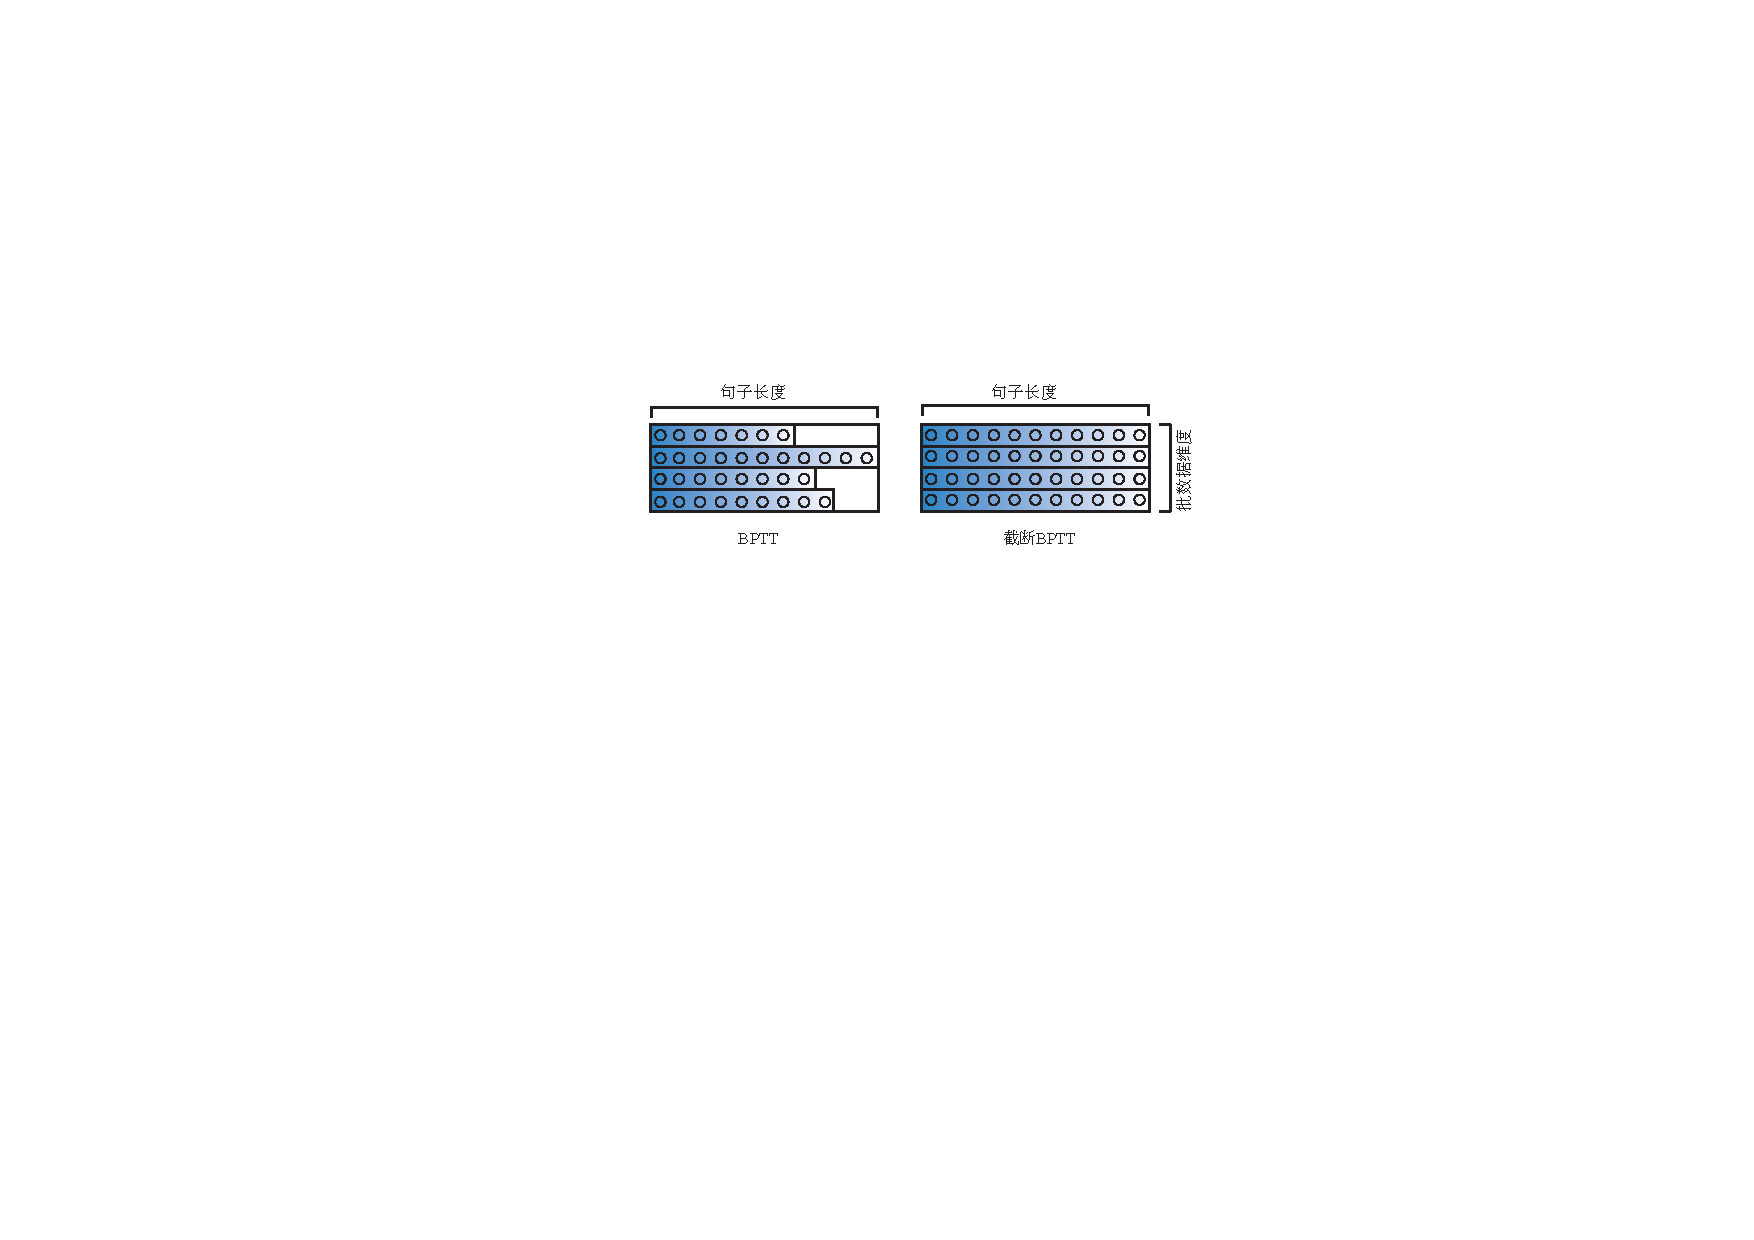
\includegraphics[width=.8\columnwidth]{./figures/minibatch.pdf}
  \caption{BPTT和截断BPTT算法示意图}\label{fig:minibatch}
\end{figure}
\begin{figure}[!t]
  \centering
  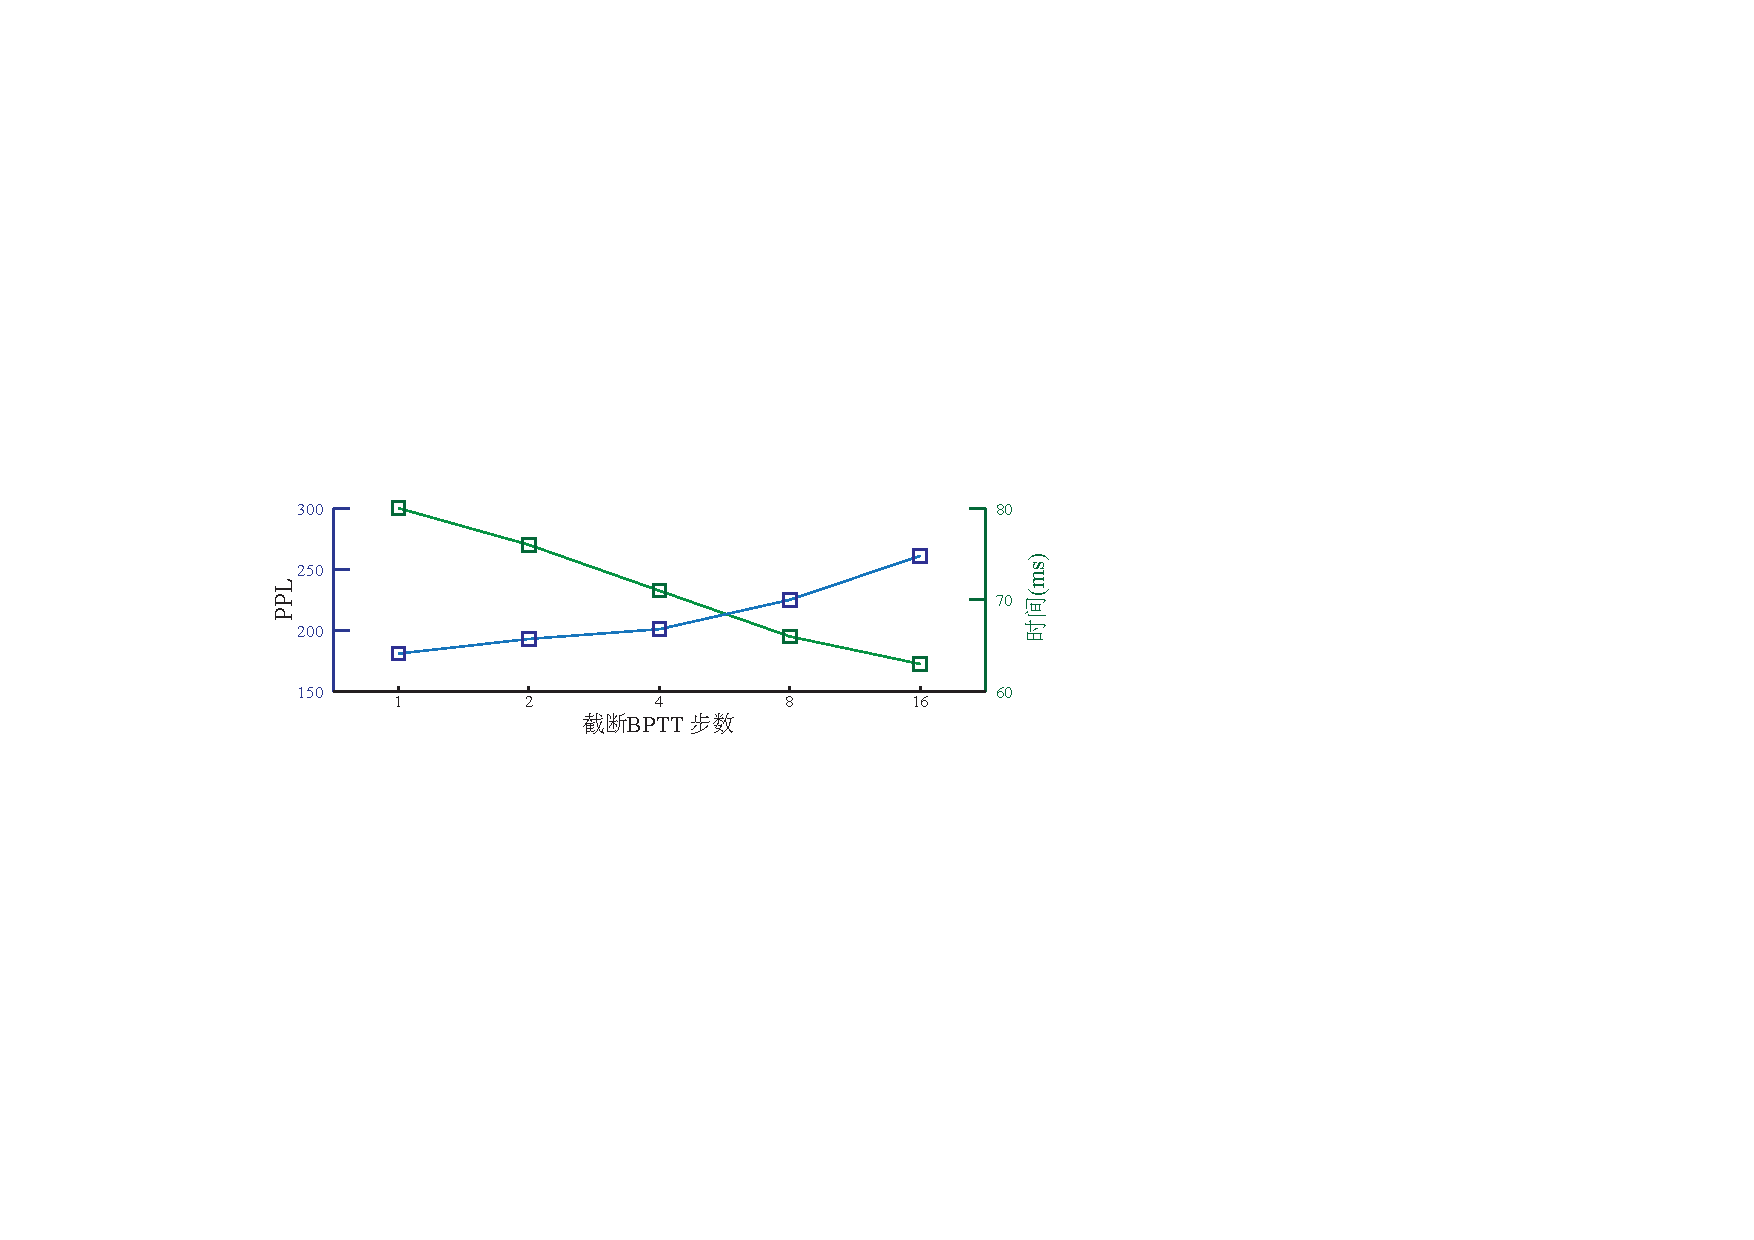
\includegraphics[width=.85\columnwidth]{./figures/tbptt.pdf}
  \caption{wikitext-2数据集上 BPTT和截断BPTT算法对RNN的影响.}\label{fig:tbptt}
\end{figure}
我们在此说明,在训练中,如果你在被截断的段中看到某些依赖关系,则可以学习它们。 如果这些依赖关系总是跨越不同的领域,我们已经打破了这些依赖关系,你永远不会学习它 因为渐变永远不会回流,并告诉前一个段中的某些内容对下一个段是有用的。 但是如果你在一个细分市场中看到他们,那么你实际上有一个希望,那就是在测试的时候,你将能够在不同的细分市场上预测它们。 因为我们总是向前传播。

\subsection{采样近似算法比较}

基于抽样的算法的效率和准确性与样本大小密切相关,我们在下一次评估中测试了这个样本。我们测试了几个样本大小,以评估它们对停电和NCE近似值的影响,结果显示在表~\ref{fig:blackout_nce}中。根据图1所示,中断算法比传统的NCE模型表现得相对较好,这与报道的实验结果是一致的~\cite{DBLP:journals/iclr/JiVSAD15}。

\begin{figure}[!t]
  \centering
  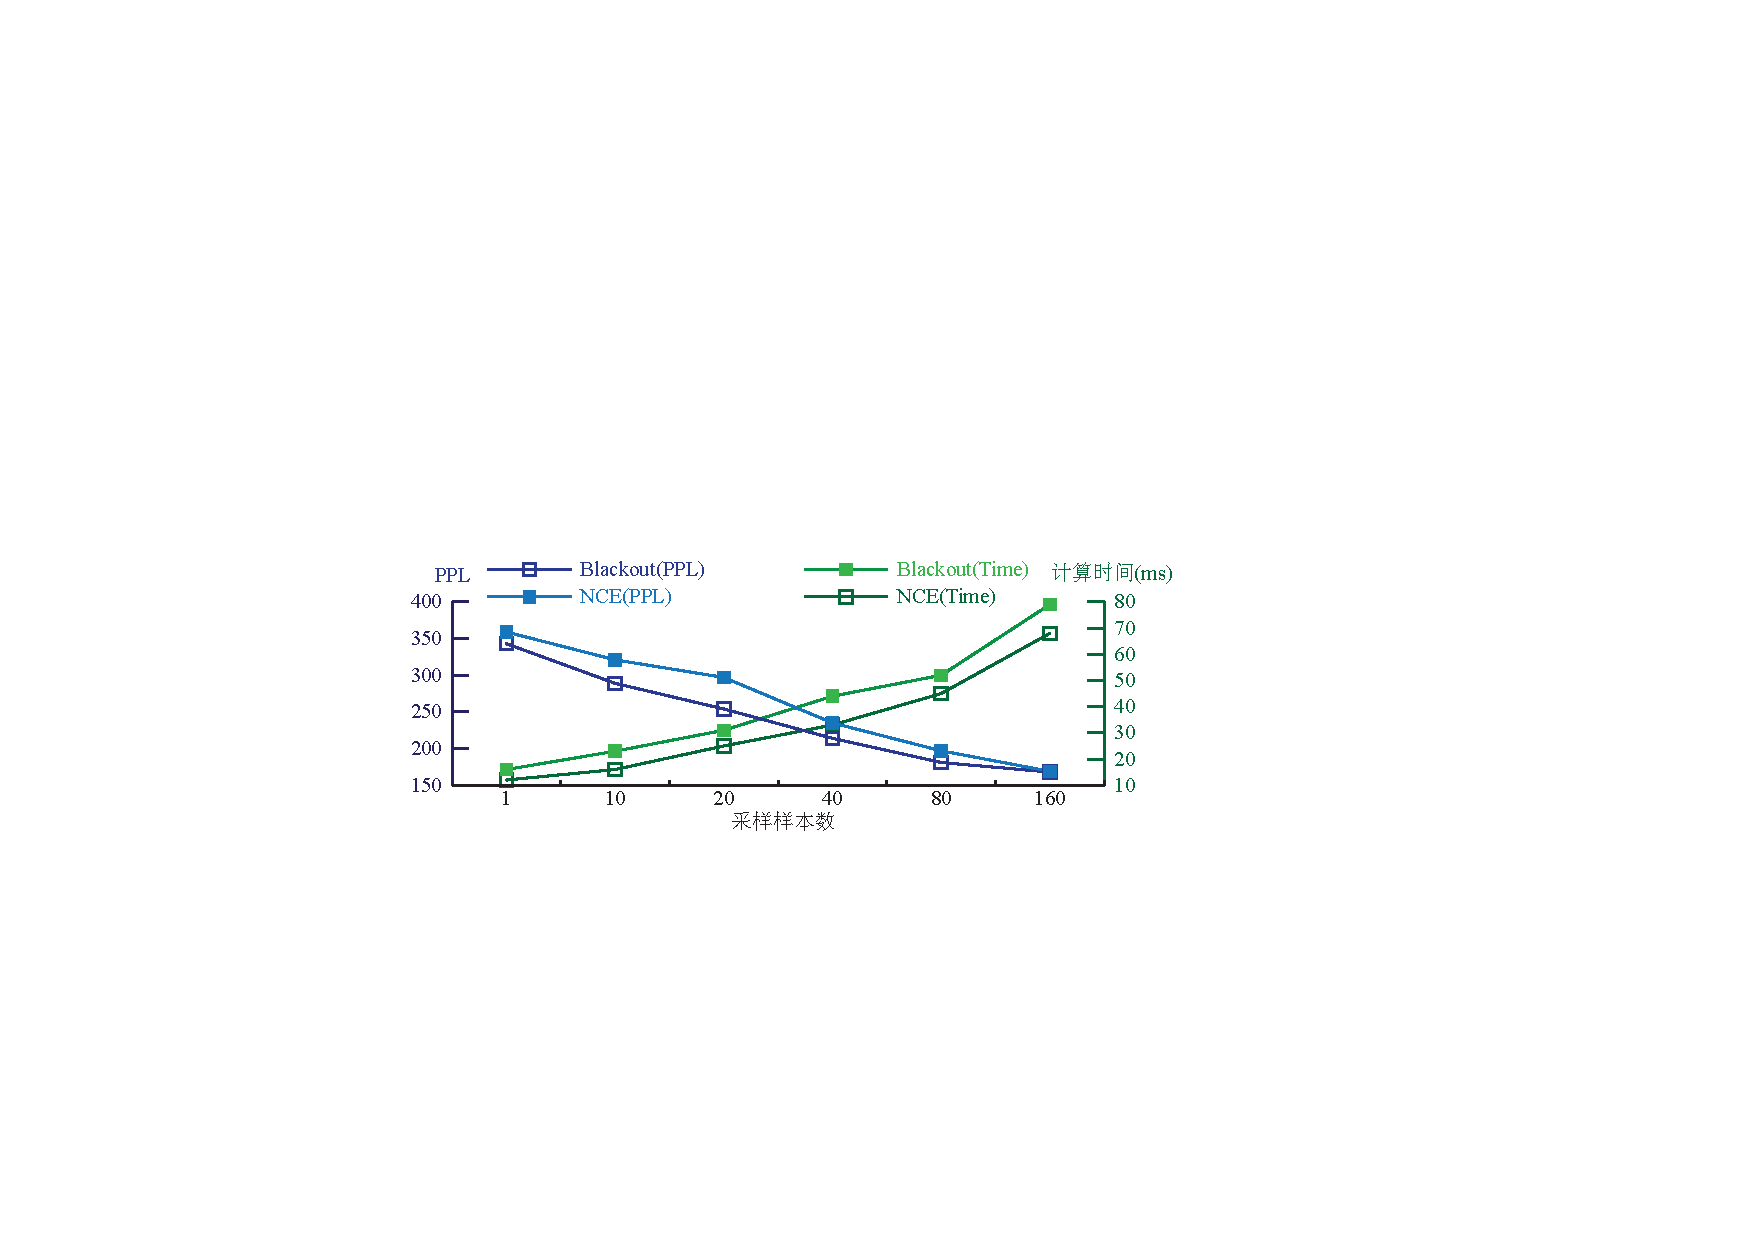
\includegraphics[width=.85\columnwidth]{./figures/nce_blackout.pdf}
  \caption{wikitext-2上测试不同采样数量对NCE和Blackout算法的影响}\label{fig:blackout_nce}
\end{figure}

我们发现一个样本大小和二元分类表现最差。训练过程涉及在真正的词概率阶段的学习,以及在噪声概率估计阶段的学习。因此,这些算法只能在收集足够的噪声样本时才能准确地估计噪声概率。这些估计算法的性能随着噪声样本数量的增加而收敛到最优混淆度,但加速比$ V / k $减小,其中$ k $表示样本大小。因此,我们把这个术语作为一个超参数,应该根据验证集进行调整,所以在训练过程中,每个特定数据集的样本量都是固定的。尽管如此,采样方法在推理过程中是不能使用的,而采用原始的softmax方法。



\subsection{单词聚类策略分析}
Chen~等人发现这个单词的层次聚类算法对cHSM算法的性能很敏感~\upcite{DBLP:conf/acl/ChenGA16}。同样,为了获得较为稳定的cHSM算法和p-HSM方法的性能,我们考虑了几个现有的聚类准则,如表~\ref{table:p-thsm}~和表~\ref{table:clustering}~所示。
\begin{table}[!t]
  \centering
   \caption{wikitext-2上评价不同聚类方法对p-HSM 算法的PPL影响\label{table:p-thsm}}
  \begin{tabular}{lcccc} \toprule
  算法  &建树时间&最大树深度 &验证集 (PPL) & 测试集 (PPL)  \\ \midrule
  Uigram  &3分钟&12 &218.42& 216.05     \\
  Bigram  &35小时&21& 186.23& 189.58\\
  Semantic &26小时 &18& \textbf{163.12} & \textbf{178.78}\\
\bottomrule
  \end{tabular}
\end{table}

\begin{table*}[!t]
  \centering
  \caption{wikitext-2数据集上不同聚类算法对cHSM 算法的PPL 和 WER 影响\label{table:clustering}}
  \begin{tabular}{lclccc} \toprule
聚类算法 & 均匀划分?&分支数& 训练轮数& 测试集 (PPL / WER)&耗时 (ms)\\ \midrule
  \multirow{6}{*}{Random}  &\multirow{6}{*}{是}&10/3330&145&211.15 / 78.55 &791\\
    &&20/1664&123&228.72 / 78.89&565\\
    &&40/832&103&234.36 / 79.21&321\\
    &&80/417&78&243.12 / 79.64&171\\
    &&160/208 &57&253.38 / 80.08&92\\
    &&182/183&48&268.63 / 80.11&88\\
  \midrule
  \multirow{6}{*}{Alphabet}  &\multirow{6}{*}{是}&10/3330 &141&199.01 / 78.07 &773\\
    &&20/1664 &120&211.34 / 78.23&551\\
    &&40/832 &100&238.75 / 79.02&313\\
    &&80/417 &90&241.75 / 79.34&174\\
    &&160/208 &56&248.35 / 79.62&97\\
    &&182/183&45&258.57 / 80.02&87\\
  \midrule
  \multirow{6}{*}{Uni-gram}   &\multirow{6}{*}{是} &10/3330&134&211.51 / 77.41 &788\\
    & &20/1664&122&220.01 / 77.71&549\\
    & &40/832&113&236.56 / 77.95&302\\
    & &80/417&91& 241.12 / 78.25&170\\
    & &160/208&55&247.25 / 79.21&93\\
    & &182/183&42&253.35 / 79.92&86\\
  \midrule
  \multirow{5}{*}{Bi-gram}   &\multirow{5}{*}{否}&10/3672&150&208.11 / 77.32&801\\
     &&20/1923&121&217,34 / 77.64&621\\
     &&40/1123&102&228.87 / 78.14&588\\
     &&80/572&89&246.32 / 78.43&186\\
     &&160/340&76&252.33 / 79.51&97\\
  \midrule
  \multirow{5}{*}{Syntactic}  &\multirow{5}{*}{否}&10/3612 &152&214.31 / 78.11&810\\
    &&20/1972 &130&220.19 / 78.86&633\\
    &&40/996 &101&232.33 / 79.33&543\\
    &&80/545 &89&241.34 / 79.84&179\\
    &&160/235 &70&262.34 / 80.14&134\\
  \midrule
  \multirow{5}{*}{Semantic}  &\multirow{5}{*}{否} &10/3570 &133&208.77 / 77.41&819\\
    & &20/1873 &114&218.31 / 77.78&641\\
    & &40/1092 &91&225.38 / 78.35&521\\
    & &80/561 &69&238.45 / 78.91&174\\
    & &160/244 &44&256.75 / 79.41&103\\
\bottomrule
  \end{tabular}
\end{table*}

一方面,我们将表~\ref{table:clustering}中的Wikitext-2数据集中,应用前面所有提到的聚类方法,同时比较了不同的分支因子对算法效果的影响,并进行了比较。从这张表中可以发现,随机洗牌方法对于其他算法的性能最差,因为它们没有提供有关先前分配的任何信息。此外,还观察到,比其他人更难以接受可接受的训练损失,因此在训练集上花费更多的时间来优化参数。然后,发现在对类结构注入外部单字和双字的知识之后,模型确实在目标空间中学习了一个明确定义的单词分布。因此,它对随机和字母表系列取得了更好的结果。而且,用语法和语义算法进行分词的词汇比上述方法得到的结果要好得多,代价是计算分割方法。从实验结果可以看出,向具有先验知识的类结构注入会增强该方法的稳定性,通过平衡聚类时间和模型的准确性,可以调整分支因子,达到预期的结果。



另一方面,我们采用了单词,字母和词汇聚类方法来生成单词在树上的分布,详细的结果在表~\ref{table:clustering}~中给出。与提供调整分支因子的自由度的cHSM方法不同,树聚类的实验是相当有限的。单字聚类(即频率合并)方法在创建单词层次结构方面效率更高,而双字词和语义聚类花费更多时间来计算词汇表中单词之间的相似度矩阵。尽管如此,考虑到树合并的规则,bigram方法考虑了二元共现统计和语义方法来评估特征空间中的欧氏距离。在困惑度量下,二元语义聚类方法比一元方法有更好的效果。最后,与cHSM方法相比,更深层次的树模型更适合于词汇聚类,适当的聚类可以提高树层次的效率。

\section{模型总体评价}
如表~\ref{tab:summary_ppl}~所示,我们收集了上述三种标准语料库的验证和测试数据集的所有困惑和错误率结果。值得注意的是,我们采用了一层GRU单元作为所有这些算法的上下文表示,其维数设置为256.另外,对于NCE和Blackout近似,超参数$ k $是 对较小的Wikitext-2和Wikitext-103数据集设置为$\mathcal{|V|}/20 $,对于较大的One Billion Word数据集,设置为$ k = | \mathcal{V} | / 200 $。 此外,对于cHSM方法,我们根据单词的单字分布来划分词汇。

考虑到Wikitext-2数据集上的结果,最初的softmax比其他算法获得了最好的分数,因为在Blackout和NCE近似中没有引入任何cHSM和p-tHSM算法的结构损失或基于抽样的变分损失。

\begin{table}[!h]
  \centering
  \caption{所有模型在三个数据集上的困惑度和单词错误率的性能评测\label{tab:summary_ppl}}
\begin{tabular}{llcc}
  \toprule
数据集& 算法& 验证集(PPL/WER) & 测试集(PPL/WER) \\ \midrule
 \multirow{2}{*}{WikiText-2}&GRU + Softmax&172.64 / 77.49\%&162.09 / 77.07\% \\
  &GRU + NCE~\upcite{DBLP:journals/jmlr/GutmannH10}&217.84 / 78.26\%&199.54 / 78.02\%\\
  &GRU + Blackout~\upcite{DBLP:journals/iclr/JiVSAD15}&221.15 / 77.72\%&199.56 / 77.50\% \\
  &GRU + cHSM + unigram~\upcite{DBLP:conf/acl/ChenGA16}&253.18 / 78.25\%&236.61 / 78.02\%\\
  &GRU + p-tHSM + unigram~\upcite{DBLP:conf/nips/MikolovSCCD13}&218.42 / 78.15\%&216.05 / 78.15\%\\
  &GRU + p-tHSM + bigram~\upcite{DBLP:journals/coling/BrownPdLM92}&186.23 / 78.15\%&189.58 / 78.15\%\\\midrule
   \multirow{2}{*}{WikiText-103} &GRU + Softmax&130.38 / 72.15\%&136.83 / 72.37\%\\
 &GRU + NCE~\upcite{DBLP:journals/jmlr/GutmannH10}&164.78 / 73.22\%&165.01 / 73.34\%\\
  &GRU + Blackout~\upcite{DBLP:journals/iclr/JiVSAD15}&163.99 / 73.18\%&162.76 / 74.22\%\\
  &GRU + cHSM + unigram~\upcite{DBLP:conf/acl/ChenGA16}&171.81 / 73.42\%&166.74 / 73.18\%\\
  &GRU + p-tHSM + unigram~\upcite{DBLP:conf/nips/MikolovSCCD13}&165.70 / 73.53\%&166.11 / 72.44\%\\
  &GRU + p-tHSM + bigram~\upcite{DBLP:journals/coling/BrownPdLM92}&164.15 / 78.15\%&163.55 / 77.85\%\\\midrule
  \multirow{2}{*}{One Billion Word} &GRU + Softmax&330.38 / 88.15\%&330.83 / 88.37\%\\
 & GRU + NCE~\upcite{DBLP:journals/jmlr/GutmannH10}&272.07 / 84.83\%&276.11 / 84.34\%\\
  &GRU + Blackout~\upcite{DBLP:journals/iclr/JiVSAD15}&268.67 / 84.23\%&266.11 / 84.18\%\\
 & GRU + cHSM + unigram~\upcite{DBLP:conf/acl/ChenGA16}&225.36 / 80.32\%&224.11 / 79.42\%\\
 & GRU + p-tHSM + unigram~\upcite{DBLP:conf/nips/MikolovSCCD13}&231.44 / 87.53\%&236.11 / 82.53\%\\
  &GRU + p-tHSM + bigram~\upcite{DBLP:journals/coling/BrownPdLM92}& 221.55 / 81.15\%&218.70 / 83.15\%\\
  \bottomrule
\end{tabular}
\end{table}

对于第二个Wikitext-103数据集,Brown聚类的p-tHSM方法不仅获得了比霍夫曼聚类方法更好的结果,而且表现也比其他方法好。另外,cHSM模型能够获得与p-tHSM变体类似的结果,表明我们可以用其他合适的用于cHSM方法的聚类算法获得更好的结果。由于Wikitext-103和Wikitext-2数据集共享相同的测试集,因此发现最初的softmax通过更大的训练数据被收敛到更好的结果。此外,对于采样方法,它收敛于比softmax方法好得多的结果,同时提高了时间效率。

综上所述,在用字极性编码方案替代tHSM中的传统霍夫曼编码方案并且实现了基于紧密的树型模型p-tHSM之后,我们证明了这种新颖的编码方案允许在GPU上并行运行计算。这将原始tHSM的时间复杂度从$ \mathcal {O(| H | \log | V |)} $减少到$\mathcal{O(| H || V |)} $并获得了最佳的加速比对于大量的词汇问题。此外,为了稳定p-tHSM模型的性能,我们测试了几种现有的层次聚类算法,发现基于树模型的词聚类与内部节点的二元分类密切相关。

\section{本章小结}

词汇量过大问题是语言模型应用中最重要的挑战之一。为了解决这个问题,文献中提出了各种方法,可大致分为三个类别:词汇截断算法,基于抽样的近似算法和词表层次分解。第一种方法易于实施,并广泛应用于实践中。而第二类可以有效地减少训练时间消耗,而不用通过重要性抽样的变化来总结所有的单词,而抽样分布的选择可以针对更稳定的结果进行优化。第三种方法将目标词汇的扁平化架构改变为具有两种可能类型的启发式分层结构:类和树因式分解。构建在两步softmax分类方法和树模型上的类方法将其扩展到$\mathcal {O(| H | \log | V |)} $步骤的二进制分类。

在这个研究中,我们不仅提出了基于二叉树或者分类层次概率模型的潜在编码方案,而且为分层softmax变体建立了并行和紧凑的损失函数。另外,利用GPU硬件的优势,可以有效地计算出目标词汇量越来越大的概率和梯度。值得注意的是,这个算法的时间复杂度超出了历史记录$ \mathcal {O(| H | \log | V |)}$,从而使它能够处理大量的词汇问题。此外,我们还扩展了几个推理策略来进行评分或排名。在实验中提出并讨论了三种算法,在分析部分中进行了很好的说明。最后,我们评估了几个单词层次聚类算法,以更有效的方式组织树中的单词。结果表明,与其他概率归一化方法相比,加速比提高,得到更高效的树聚类,与其他基于抽样的优化相比,性能相对较好。

在未来的研究中,我们计划探索softplus函数的应用场景,并探讨在cHSM算法训练的时候的词表动态交换算法。另外,实验中应用的几种聚类算法消耗了很多时间,我们可以优化该聚类算法,设计更高效的分层结构。
